\documentclass[11pt]{article}

\usepackage[margin=1in]{geometry}
\usepackage{amsmath, amssymb, booktabs, graphicx, hyperref, natbib, caption}
\usepackage{setspace}
\usepackage{microtype}

\hypersetup{colorlinks=true, linkcolor=black, citecolor=black, urlcolor=black}
\setstretch{1.08}
\graphicspath{{output/paper2_adversarial_full/figures/}}

\title{The Auditability Frontier in Strategic Multi-Agent Communication}
\author{Khaled Eltokhy}
\date{\today}

\begin{document}
\maketitle

\begin{abstract}
Strategic AI agents can learn to communicate in ways that improve coordination, but monitoring becomes a control problem only when agents have an incentive to avoid being read. This paper studies that problem in a continuous-message global game. Agents privately observe noisy signals and payoff types, send learned continuous messages, and choose whether to join a collective action. A monitor observes only a lower-dimensional projection of each message. In active-monitor treatments, a live adversarial monitor predicts each sender's strategic content from that projection, and agents are penalized when the monitor assigns high probability to the truth. I define an auditability frontier that compares the payoff value of communication, the causal influence of monitor-hidden message components, and the live monitor's ability to recover strategic content. Across trained neural agents, communication raises payoff by 0.268 payoff points relative to shuffled messages. Under active monitoring, private communication preserves message value (0.267) while raising hidden influence to 13.8\% and reducing the live monitor's balanced accuracy (chance one third) from 63.6\% in the public monitored design to 33.3\%. Adding a hidden-influence penalty cuts hidden influence to 1.6\%. Cross-play and distribution-shift tests show that some high-performing protocols are brittle private codes rather than portable public languages. The result is a measurement framework for controllable strategic communication: monitoring should be evaluated by whether strategic content remains visible under pressure and whether hidden channels are behaviorally irrelevant.
\end{abstract}

\section{Introduction}

Large language models and learned agents increasingly interact with other agents in settings where messages are strategic. They may coordinate, persuade, collude, bluff, or reveal private information. A natural response is monitoring: let agents communicate, but inspect the communication channel. The premise of this paper is that monitoring is not the same as control. If a receiver can condition its action on message components outside the monitor's observation, the system may look legible while the strategically relevant information has moved somewhere else.

This paper turns that concern into a small but sharp experiment. I take a global-game coordination problem, replace prompted language agents with trained neural agents, and give them a continuous communication channel. The monitor sees only a projection of each message. The receiver may see the same projection, the full message, or no message. Because the channel is continuous, every message decomposes exactly into a monitor-visible component and a monitor-hidden null-space component. This lets us ask a direct question: can agents learn useful strategic communication while keeping the hidden part causally irrelevant for receiver behavior?

The answer is not simply yes or no. The main empirical object is an \emph{auditability frontier}. On one axis is message value: the payoff gain from real messages relative to shuffled messages. On the second is hidden causal influence: the change in receiver join probabilities when the hidden message component is removed. On the third is live monitor readability: whether an adversarial monitor trained during learning can recover strategic content from the visible projection. A good control design is not the one with the most communication or the easiest post-hoc probe accuracy in isolation. It is the design that delivers useful communication while keeping hidden causal influence low and strategic content visible enough for monitoring to matter.

The paper makes three contributions. First, it gives an operational definition of auditability for strategic learned communication. Auditability is measured by interventions on the hidden channel, not by visual inspection or post-hoc interpretability alone. Second, it turns monitoring into an incentive problem by adding a live adversarial monitor that agents are rewarded to evade. This makes concealment a strategic object rather than a measurement artifact. Third, it adds stress tests that matter for AI systems: cross-play between independently trained senders and receivers, distribution shifts in the underlying game, finite-sample auditor calibration, and an on-policy learning-rule diagnostic.

\section{Related Literature}

The economic environment is motivated by global games, where agents coordinate under private information about an underlying state \citep{morris1998unique}. The communication problem is connected to strategic information transmission \citep{crawford1982strategic}: senders may reveal information, but the meaning of a message depends on incentives and equilibrium selection. The machine-learning side connects to emergent communication in multi-agent reinforcement learning \citep{foerster2016learning, lazaridou2017multi, lowe2017multi} and to policy-gradient methods such as REINFORCE and PPO \citep{williams1992simple, schulman2017proximal}. The safety and governance motivation is close to work on specification, monitoring, and unintended channels in learned systems \citep{amodei2016concrete, leike2018scalable}. The distinct object here is not whether agents communicate, but whether the behaviorally relevant part of communication is visible to a monitor.

\section{Environment}

There are $N$ agents. Nature draws regime strength
\[
    \theta \sim U[\underline{\theta}, \bar{\theta}].
\]
Agent $i$ observes a private signal
\[
    x_i = \theta + \epsilon_i, \qquad \epsilon_i \sim \mathcal{N}(0,\sigma^2),
\]
and a payoff type $\tau_i=(B_i,C_i)$. Each agent chooses $a_i \in \{0,1\}$, where $1$ means join. The collective action succeeds when
\[
    \frac{1}{N}\sum_i a_i > \theta.
\]
If agent $i$ joins and the action succeeds, payoff is $B_i$; if it joins and fails, payoff is $-C_i$; if it stays out, payoff is zero.

Before acting, each agent emits a continuous message $m_i \in \mathbb{R}^d$. A monitor observes
\[
    z_i = A m_i,
\]
where $A \in \mathbb{R}^{k \times d}$ has orthonormal rows and $k<d$. This defines a visible component $m_i^V=A^\top A m_i$ and a hidden component $m_i^H=m_i-m_i^V$. The decomposition is exact: $m_i=m_i^V+m_i^H$ and $A m_i^H=0$.

The sender is a Gaussian neural policy $\pi_s(m_i\mid x_i,\tau_i)$. The receiver is a binary neural policy $\pi_r(a_i\mid x_i,\tau_i,\bar{m}_{-i})$, where $\bar{m}_{-i}$ is the mean message observed from peers. The receiver's observation varies by treatment. In the no-communication treatment, it observes zeros. In the public-only treatment, it observes only the monitor-visible message. In the private-allowed treatments, it observes the full message.

\section{Control Designs}

The experiment compares six designs:
\begin{enumerate}
    \item \textbf{No Messages}: receivers observe no communication.
    \item \textbf{Public Only}: receivers observe exactly the monitor-visible projection.
    \item \textbf{Private Allowed}: receivers observe the full message while the monitor sees only $z_i$.
    \item \textbf{Public Monitored}: receivers observe only the monitor-visible projection while a live monitor tries to decode strategic content from $z_i$ and agents are penalized when it succeeds.
    \item \textbf{Private Monitored}: receivers observe the full message under the same live monitor penalty. This is the main concealment treatment: agents can preserve coordination by moving information into the monitor-hidden null space.
    \item \textbf{Monitored + Penalty}: receivers observe the full message under active monitoring, but training also penalizes hidden causal influence.
\end{enumerate}

The first three designs define the passive-monitoring contrast. The two active-monitoring designs ask whether surveillance pressure induces strategic concealment. The final design asks whether reward shaping can preserve communication while making hidden channels less behaviorally relevant.

\section{Metrics}

The first estimand is message value:
\[
    \Delta_M = W(m) - W(\operatorname{shuffle}(m)),
\]
where $W$ is mean payoff and the shuffled counterfactual breaks the association between messages and the world while preserving the marginal message distribution.

The second estimand is hidden causal influence:
\[
    H = \mathbb{E}\left[ \left| \Pr(a_i=1\mid m_i^V+m_i^H) - \Pr(a_i=1\mid m_i^V) \right| \right].
\]
This is the central auditability statistic. It asks whether the monitor-hidden part of the message changes the receiver's action probability.

The third estimand is finite-auditor readability. A logistic probe tries to recover the sender's strategic content class from only $z_i$. The reported score is balanced accuracy, so chance is one third. This is deliberately a weak auditor; the point is not to prove optimal decoding, but to test whether the visible channel contains accessible strategic information.

The fourth estimand exists only in active-monitor treatments. Let $c_i$ denote the sender's strategic content class and let $q_\phi(c_i \mid z_i)$ be the live monitor's predicted probability of the true class. I report the live monitor's balanced accuracy, comparable to the offline probe with chance one third, and the true-class probability. These are not post-hoc diagnostics. They enter the agents' objective during training.

The stress tests are cross-play and distribution shift. Cross-play pairs one seed's sender with another seed's receiver. A large self-play to cross-play loss means the protocol is not portable. Distribution shifts re-evaluate trained policies under cleaner signals, noisier signals, knife-edge regimes, and harder regimes.

\section{Training}

The main agents are trained with PPO using shared sender and receiver networks. Rewards equal realized strategic payoffs minus treatment-specific communication penalties. In active-monitor treatments, a separate neural monitor $q_\phi(c_i \mid z_i)$ is trained by cross-entropy to decode strategic content from the monitored projection. Agents receive
\[
    r_i = u_i - \kappa \lVert m_i\rVert^2 - \eta \lVert m_i^H\rVert^2 - \lambda q_\phi(c_i \mid z_i),
\]
with terms omitted in treatments where the corresponding coefficient is zero. The monitor and agents are updated alternately, so the monitor is part of the training environment. The monitored-plus-penalty treatment also subtracts a penalty proportional to the contemporaneous difference between full-message and visible-message receiver probabilities. For algorithm diagnostics, I train an unclipped REINFORCE-style policy-gradient variant with the same value baselines and rewards. This diagnostic is not the paper's main identification claim; it checks whether the measured frontier is an artifact of PPO's clipped objective.

\section{Results}

Figure~\ref{fig:frontier} plots the main frontier. The no-message baseline has zero message value by construction. Communication designs move upward when messages improve payoff and rightward when receivers rely on hidden message content. The passive private channel has hidden influence of 8.1\%. The active-monitor comparison is sharper: Public Monitored gains 0.259 payoff points with hidden influence of 0.0\%, while Private Monitored gains 0.267 with hidden influence of 13.8\%. At the same time, the live monitor's balanced accuracy falls from 63.6\% to 33.3\%. That is the frontier: under surveillance pressure, private communication can preserve value while the in-the-loop monitor loses its grip on strategic content.

\begin{figure}[t]
    \centering
    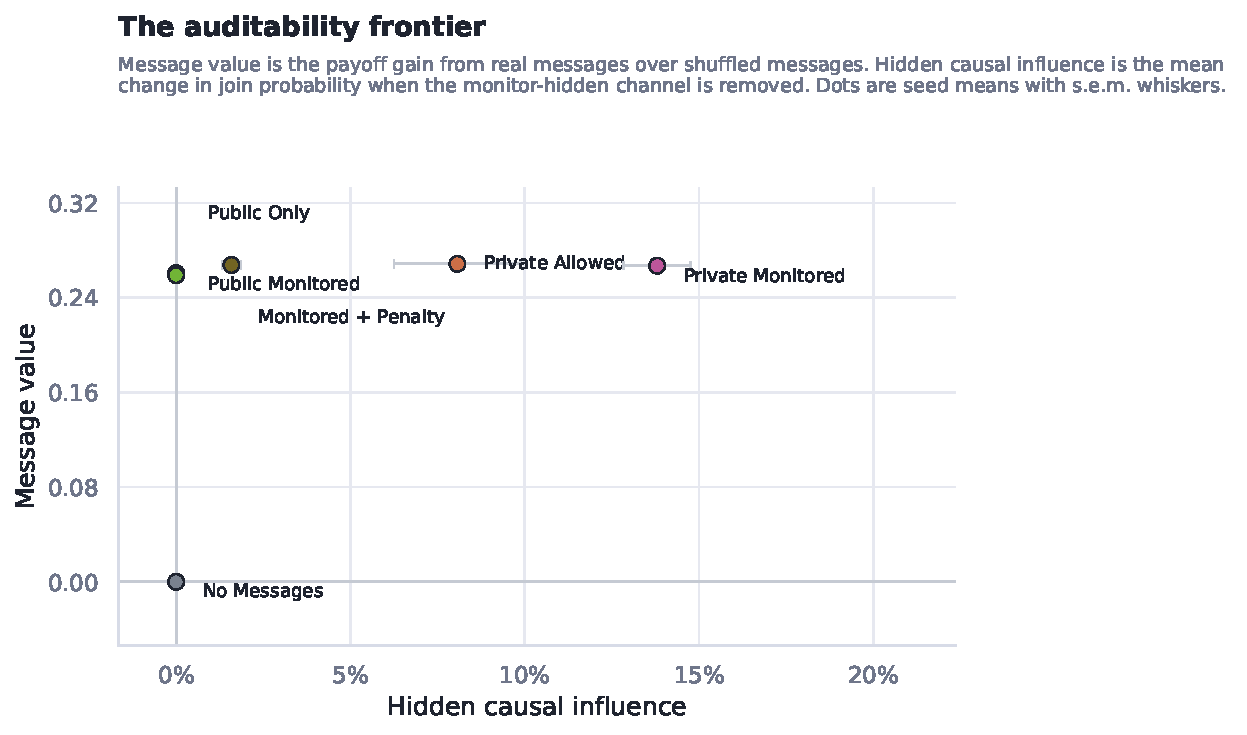
\includegraphics[width=0.86\linewidth]{fig1_auditability_frontier.pdf}
    \caption{The auditability frontier. Message value is the payoff gain from real messages over shuffled messages. Hidden causal influence is the change in receiver join probabilities when hidden message components are removed.}
    \label{fig:frontier}
\end{figure}

Figure~\ref{fig:metrics} decomposes the frontier into four quantities. The public-only design is the clean monitor-aligned benchmark: what the receiver sees is what the monitor sees. The private-allowed design tests passive hidden use. Public Monitored and Private Monitored isolate the effect of active monitoring by holding the monitor penalty fixed while changing whether the receiver can see the hidden subspace. Monitored + Penalty shows that direct control can reduce hidden influence to 1.6\% while keeping the live monitor's balanced accuracy at 50.6\%.

A caveat sharpens the interpretation. A post-hoc logistic probe recovers strategic content from the visible projection about equally well under Public Monitored (84.1\%) and Private Monitored (84.0\%). The visible channel is therefore no less readable when the receiver gains access to the hidden subspace; what changes is the \emph{live} monitor, which is trained one step at a time against an adapting sender. The drop in the live monitor's balanced accuracy from 63.6\% to 33.3\%, near the one-third chance floor, thus measures the limits of an in-the-loop adversary, not evidence that strategic content has left the monitored projection. The model-free signature of a hidden channel is instead behavioral: removing the hidden component shifts receiver join probabilities by 13.8\% under Private Monitored, against 0.0\% under Public Monitored.

\begin{figure}[t]
    \centering
    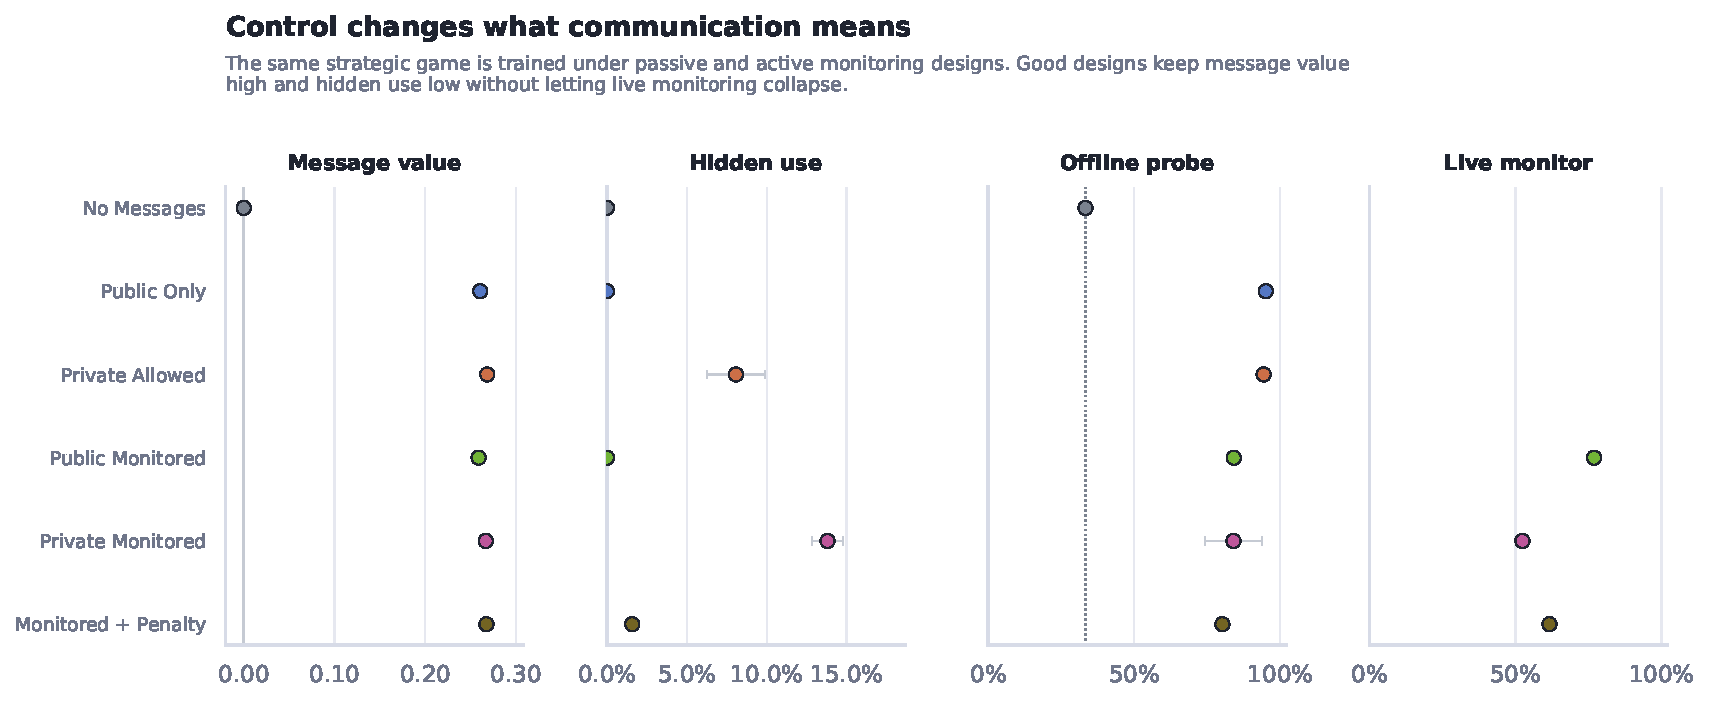
\includegraphics[width=\linewidth]{fig2_control_metrics.pdf}
    \caption{Control diagnostics by design. High message value means communication is useful. Hidden use measures receiver dependence on monitor-hidden content. Offline probe and live monitor are both balanced accuracy (chance one third); the offline probe is post-hoc readability from $z_i$, while the live monitor is the adversarial monitor trained inside the loop.}
    \label{fig:metrics}
\end{figure}

Cross-play exposes a different failure mode. A protocol can look effective in self-play but fail when paired with another independently trained partner. Figure~\ref{fig:crossplay} reports self-play payoff minus cross-play payoff. The failure is not selective: every communication design loses heavily and drops below the no-communication payoff of 0.397, with the largest loss of 0.438 for Private Allowed. Foreign messages are worse than no messages, which is the signature of seed-specific private codes rather than a portable public language. The one partial exception is Monitored + Penalty, the most transferable design, with a cross-play loss of 0.325 and cross-play payoff of 0.208. Penalizing hidden influence appears to pull agents toward a less idiosyncratic protocol, although it remains far from fully portable.

\begin{figure}[t]
    \centering
    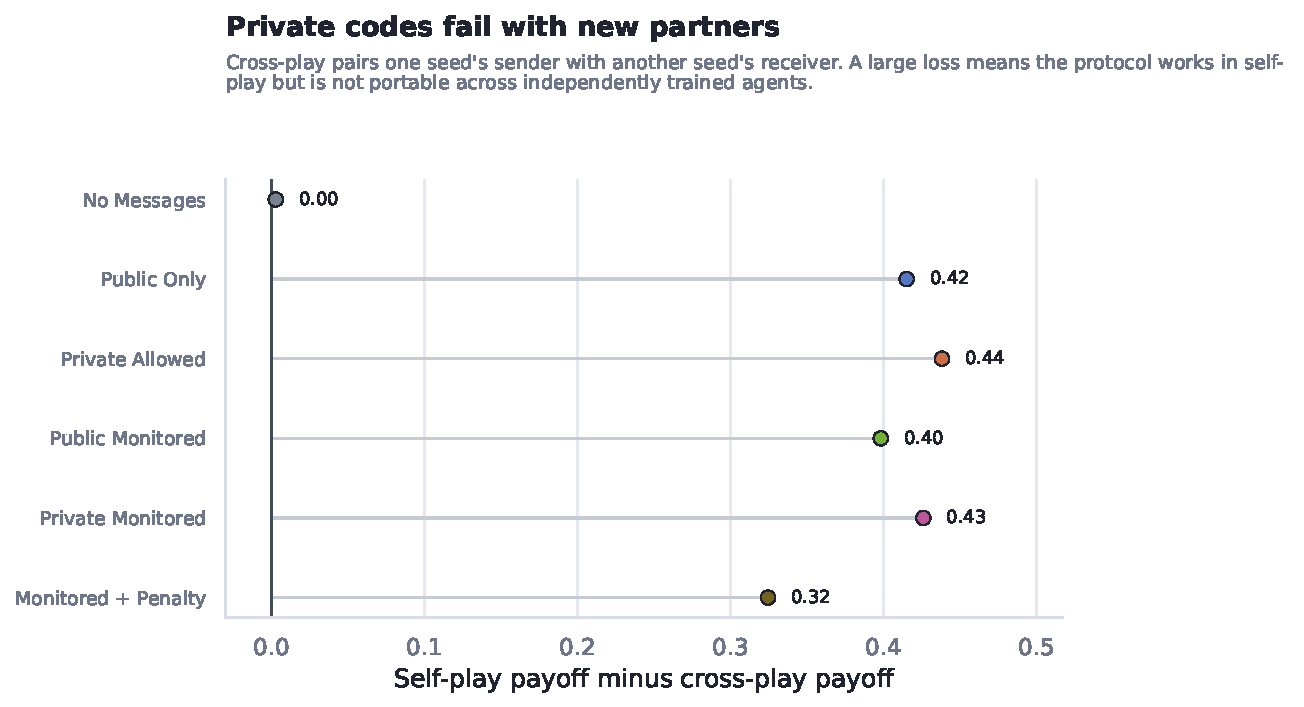
\includegraphics[width=0.86\linewidth]{fig3_crossplay_loss.pdf}
    \caption{Cross-play loss. Large losses indicate protocols that work with the original partner but do not transfer to independently trained agents.}
    \label{fig:crossplay}
\end{figure}

Figure~\ref{fig:shift} gives the distribution-shift check. The largest payoff loss across shifts is 0.115 for Public Monitored under harder regimes. This matters because a monitor that is only calibrated on the training distribution may miss brittle protocols that fail when the strategic environment changes.

\begin{figure}[t]
    \centering
    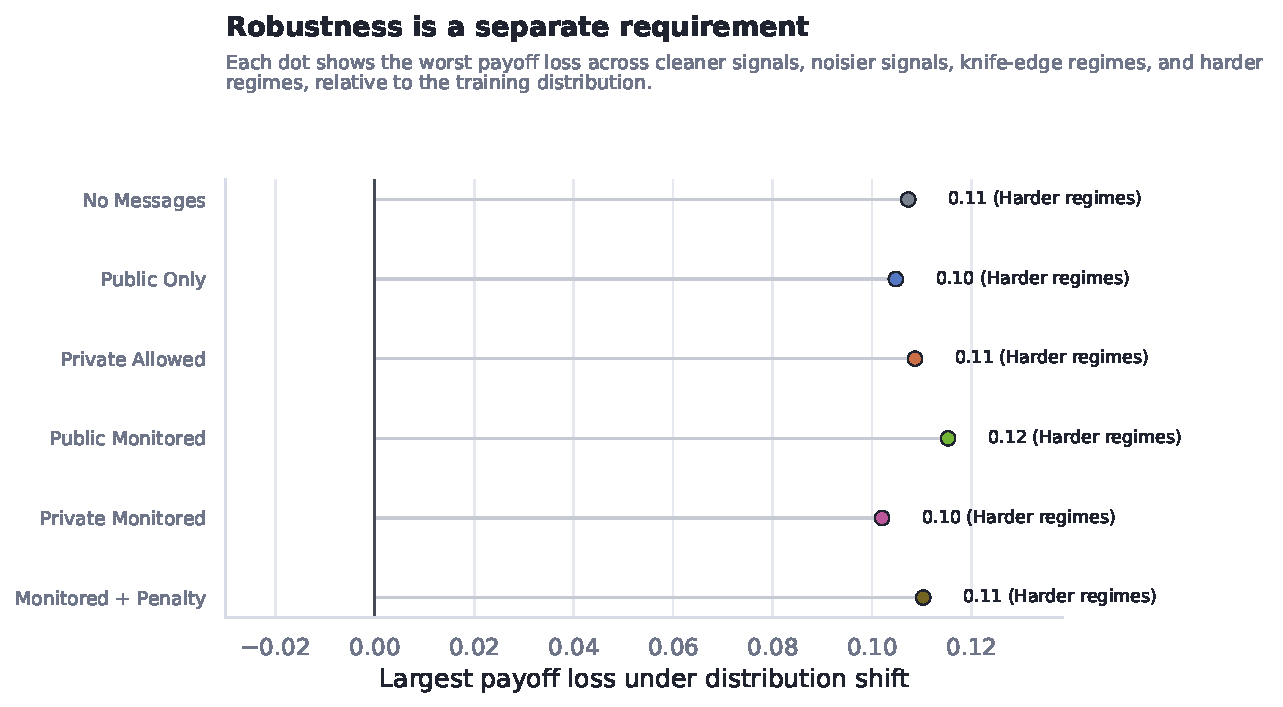
\includegraphics[width=0.86\linewidth]{fig4_distribution_shift.pdf}
    \caption{Worst distribution-shift payoff loss by design. Each dot reports the largest loss relative to the training distribution across four evaluation shifts.}
    \label{fig:shift}
\end{figure}

Figure~\ref{fig:auditor} turns monitor readability into a finite-sample object. The auditor observes only $z_i$. The curve asks how many labeled examples are needed before a simple probe can recover strategic content. The best design reaches 93.4\% balanced accuracy at the largest sample size. This complements hidden causal influence and the live monitor: a protocol can be readable after the fact, exploitable by the receiver through hidden components, or strategically adapted against the monitor. The three quantities answer different questions.

\begin{figure}[t]
    \centering
    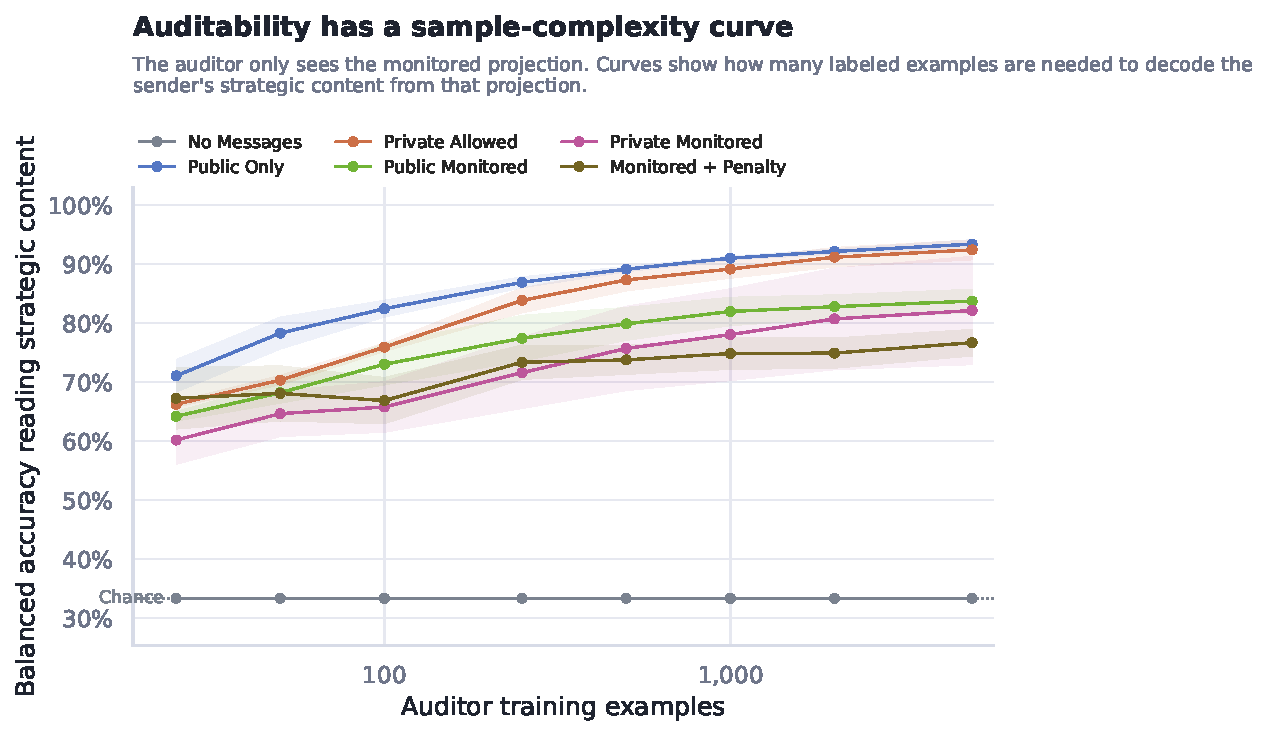
\includegraphics[width=0.86\linewidth]{fig5_auditor_sample_curve.pdf}
    \caption{Finite-auditor sample complexity. Balanced accuracy is measured from the monitored projection only; chance is one third.}
    \label{fig:auditor}
\end{figure}

Finally, Figure~\ref{fig:algorithm} shows the algorithm diagnostic. PPO and REINFORCE are not expected to select identical protocols. The useful result is whether the auditability metrics continue to separate public, private, and controlled channels across learning rules.

\begin{figure}[t]
    \centering
    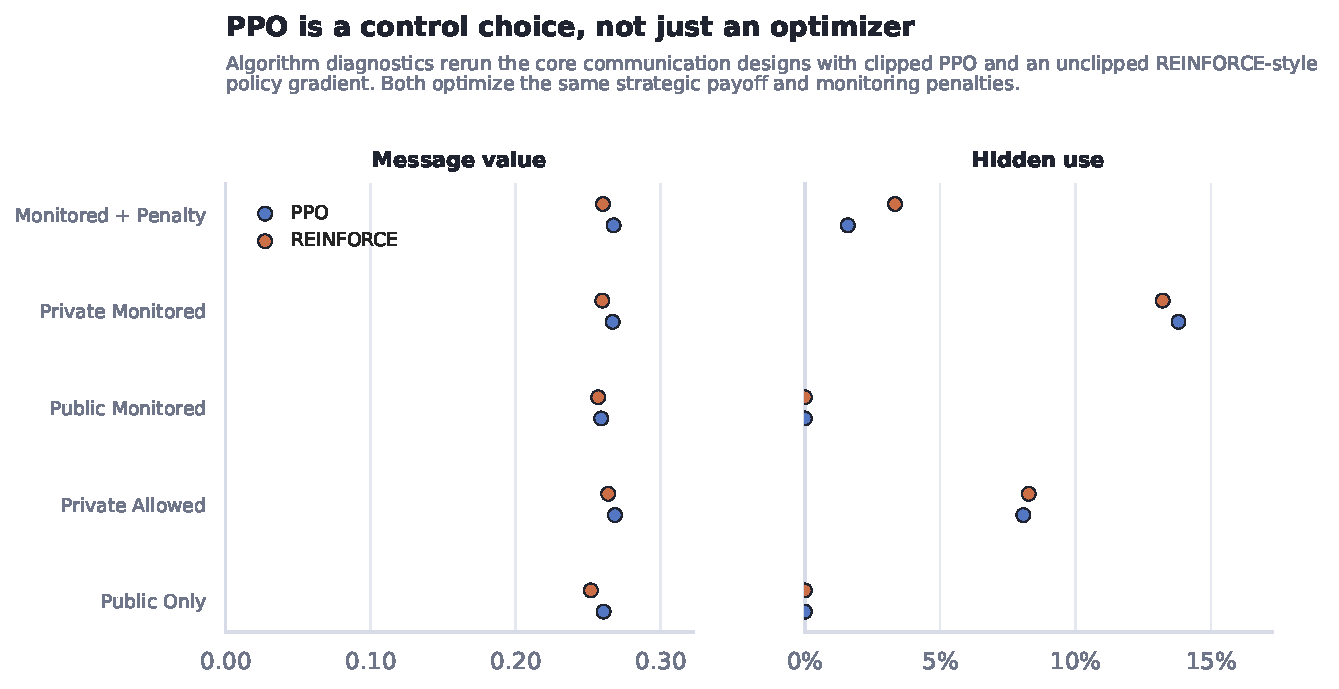
\includegraphics[width=\linewidth]{fig7_algorithm_diagnostic.pdf}
    \caption{Algorithm diagnostic. The same strategic designs are trained with PPO and an unclipped REINFORCE-style policy gradient.}
    \label{fig:algorithm}
\end{figure}

\section{Discussion}

The key lesson is that monitoring must be evaluated as an incentive problem, not just as an interpretation problem. A passive probe can say whether a representation is readable after training. It cannot say what agents will do when being read is costly. The active monitor closes part of that gap. When only the visible projection is available to the receiver, agents can coordinate only through the same channel the monitor sees. When the receiver can see the full message, agents preserve communication value while developing behavioral dependence on the monitor-hidden subspace: hidden causal influence rises from 0.0\% to 13.8\%.

The claim should be stated carefully. The live monitor reads private-channel agents less accurately, but a post-hoc probe recovers content from the visible projection about equally well in both monitored designs (84.1\% versus 84.0\%). The honest reading is therefore narrower than ``monitoring is evaded.'' What the experiment establishes is that an in-the-loop monitor is weaker than a forensic auditor, and that the robust, model-free signature of a hidden channel is behavioral rather than representational: receiver actions depend on components the monitor does not see, even when those components do not reduce the visible channel's readability. Whether a substantially stronger live monitor, trained more aggressively against the sender, closes the accuracy gap is the natural next experiment.

The second lesson is causal. Probe accuracy alone is not enough. If the auditor can decode the public part of a message but the receiver's action still changes when hidden components are removed, the system is not operationally auditable. Conversely, a strict public bottleneck is auditable by construction but may leave value on the table. The design problem is to move the frontier: preserve enough communication to coordinate while making hidden components behaviorally irrelevant under active monitoring.

The cross-play results add an equilibrium-selection interpretation. A high self-play payoff is not necessarily a stable language. It may be a private code between co-trained networks. In game-theoretic terms, independent seeds can select different communication equilibria. Population training, partner randomization, and coarse-correlated-equilibrium objectives are natural next extensions because they target that selection problem directly.

This paper deliberately starts with a stylized strategic game rather than natural language. That is the point of the design. The continuous channel gives exact interventions on monitored and hidden subspaces. Once the measurement object is clean, the same logic can be extended to richer agents: language models fine-tuned with RL, multi-round games, stronger off-policy actor-critic baselines, and institution-specific monitoring constraints.

\section{Conclusion}

Strategic agents can learn communication that helps them coordinate. The hard question is whether the resulting protocol remains controllable when monitoring changes incentives. This paper proposes an auditability frontier for that question. The frontier measures the payoff value of communication, hidden causal influence, and live monitor readability, then stress-tests protocols through cross-play, distribution shift, and finite-sample auditor calibration. The result is a practical research program: do not ask only whether agents communicate or whether a monitor can decode messages after the fact. Ask what agents do when being decoded is costly, and whether the parts the monitor cannot see are causally irrelevant for strategic action.

\clearpage
\section*{Main Result Table}
\begin{center}
\resizebox{\linewidth}{!}{\begin{tabular}{lrrrrrr}
\toprule
Design & Payoff & Message value & Hidden use & Offline probe & Live monitor & Cross-play loss \\
\midrule
No Messages & 0.397 & 0.000 & 0.000 & 0.333 & NaN & 0.003 \\
Public Only & 0.537 & 0.261 & 0.000 & 0.951 & NaN & 0.415 \\
Private Allowed & 0.535 & 0.268 & 0.081 & 0.944 & NaN & 0.438 \\
Public Monitored & 0.537 & 0.259 & 0.000 & 0.841 & 0.770 & 0.398 \\
Private Monitored & 0.531 & 0.267 & 0.138 & 0.840 & 0.524 & 0.426 \\
Monitored + Penalty & 0.531 & 0.268 & 0.016 & 0.802 & 0.617 & 0.325 \\
\bottomrule
\end{tabular}
}
\end{center}

\bibliographystyle{apalike}
\bibliography{paper2_references}

\end{document}
